% Block-Structured Quad Meshing of Turbomachinery Surfaces -- showcase deck.
% Build:  pdflatex presentation.tex   (run twice for the outline/nav)
% Theme:  Boadilla ships with beamer. For the metropolis look instead,
%         install texlive's beamertheme-metropolis and swap the \usetheme line
%         (\usetheme{metropolis}); the rest compiles unchanged.
\documentclass[aspectratio=169]{beamer}
\usetheme{Boadilla}
\usecolortheme{whale}
\usepackage{amsmath, amssymb}
\usepackage[T1]{fontenc}
\usepackage{graphicx}
\graphicspath{{figures/}}

\setbeamertemplate{navigation symbols}{}
\setbeamertemplate{caption}{\raggedright\insertcaption\par}

\title[Domain Partition]{Block-Structured Quad Meshing of Turbomachinery Surfaces}
\subtitle{A cross-field guided domain-partition pipeline}
\author{Domain-Partition 3D}
\date{\today}

% Reusable footer citation line
\newcommand{\srcline}[1]{{\footnotesize\textcolor{gray}{#1}}}

\begin{document}

\begin{frame}
  \titlepage
\end{frame}

% ---------------------------------------------------------------------------
\begin{frame}{Goal \& Pipeline}
  \begin{columns}[T]
    \begin{column}{0.54\textwidth}
      \textbf{Goal:} turn a raw turbine hub/shroud surface into a
      \emph{block-structured, all-quad} mesh suitable for CFD.

      \vspace{0.6em}
      \textbf{Pipeline:}
      \begin{enumerate}\small
        \item Unwrap cylinder $\rightarrow$ 2D
        \item Cross-field (quad orientation)
        \item Singularities
        \item Streamlines / separatrices
        \item Simplify \& partition into blocks
        \item Fill blocks with a structured grid
      \end{enumerate}
    \end{column}
    \begin{column}{0.46\textwidth}
      \centering
      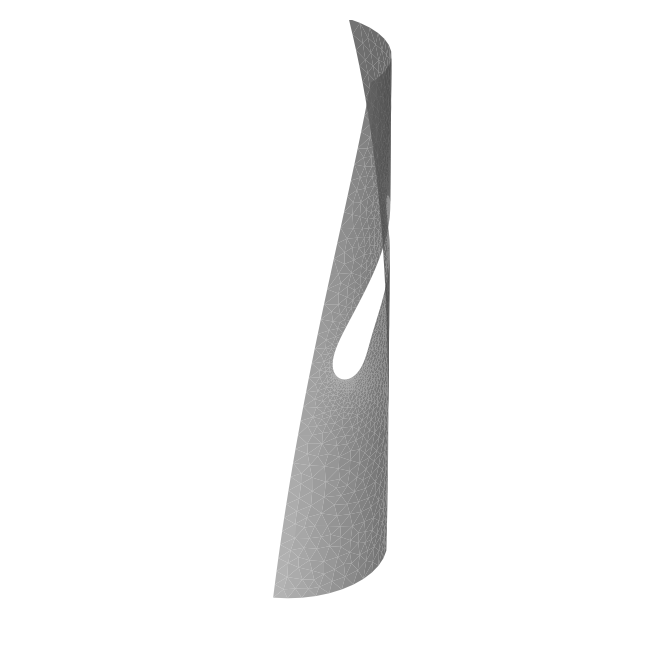
\includegraphics[height=0.72\textheight]{step01_3d_surface_hub.png}\\
      \srcline{T1\_9 turbine hub (cylindrical surface)}
    \end{column}
  \end{columns}
\end{frame}
\note{Motivation: CFD on turbomachinery wants block-structured quad meshes for
accuracy and periodic boundaries. The input is a raw triangulated hub or
shroud surface; the pipeline is fully automatic. Walk the six stages; the
following slides take one each. Only the hub runs cleanly today; the shroud
is work in progress.}

% ---------------------------------------------------------------------------
\begin{frame}{Step 1 --- Unwrap the Cylinder}
  \begin{columns}[T]
    \begin{column}{0.58\textwidth}
      \[
        \theta = \operatorname{atan2}(y,x),\quad
        s = r\,\theta,\quad t = z
      \]
      \begin{itemize}
        \item Constant radius $\Rightarrow$ \textbf{isometric} (distortion-free)
        \item 2D triangulation identical to 3D --- only coordinates change
        \item Sheared strip with a blade-shaped hole; the two
              $\theta$-walls are \textbf{periodic} (one blade pitch apart)
      \end{itemize}
      \vspace{0.5em}
      \srcline{Code: \texttt{dp3d/unwrap\_surface.py}}
    \end{column}
    \begin{column}{0.42\textwidth}
      \centering
      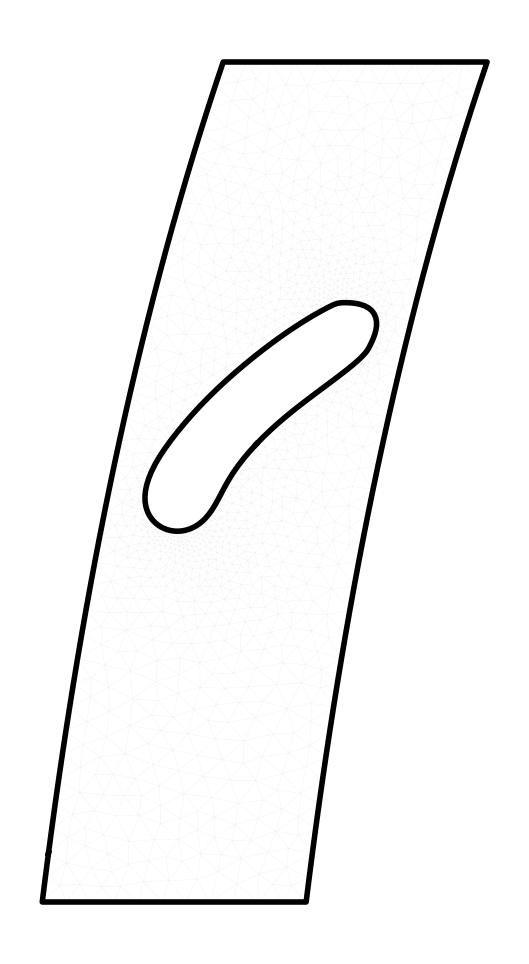
\includegraphics[height=0.74\textheight]{step02_unwrapped_hub.png}
    \end{column}
  \end{columns}
\end{frame}
\note{The hub is an exact cylinder, so mapping to arc length s and axial z is
isometric: no distortion, the mesh connectivity is untouched. We now have the
standard 2D domain-partition problem: a sheared strip with a blade hole and a
periodic pair of theta-walls one pitch apart.}

% ---------------------------------------------------------------------------
\begin{frame}{Step 2 --- Cross-Field (Quad Orientation)}
  \begin{columns}[T]
    \begin{column}{0.58\textwidth}
      \[
        \mathbf{c}(x)=\bigl(\cos 4\theta(x),\ \sin 4\theta(x)\bigr)
      \]
      \begin{itemize}
        \item \textbf{4-RoSy} field: four directions per point, invariant
              under $90^\circ$ rotation --- exactly a quad's axes
        \item Smoothed by a harmonic solve, aligned to the walls
        \item A \emph{representative vector} picks one of the four to
              integrate along
      \end{itemize}
      \vspace{0.5em}
      \srcline{Kn\"oppel et al., ``Globally Optimal Direction Fields'',
               SIGGRAPH 2013}
    \end{column}
    \begin{column}{0.42\textwidth}
      \centering
      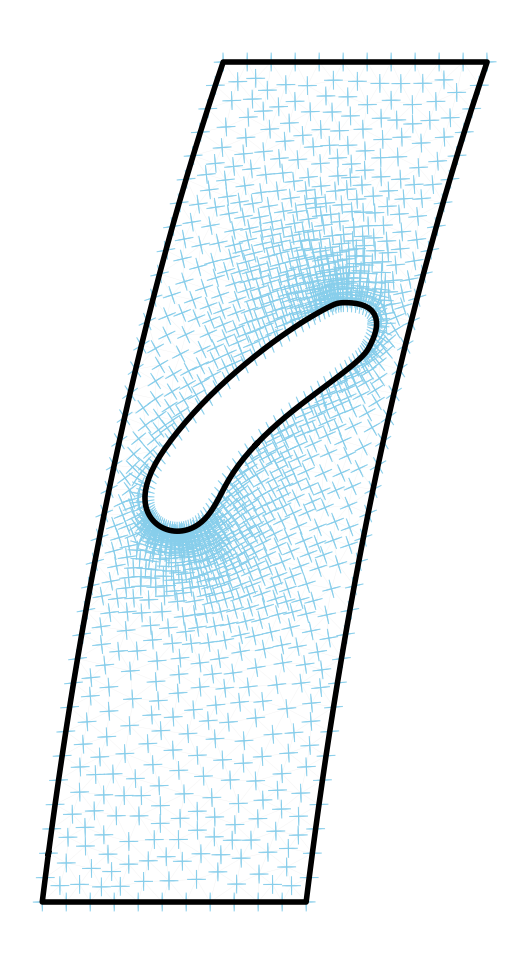
\includegraphics[height=0.74\textheight]{step05_framefield_hub.png}
    \end{column}
  \end{columns}
\end{frame}
\note{The cross-field says how quads should be oriented everywhere. 4-RoSy means
four-fold rotational symmetry: at each point four directions 90 degrees apart,
which is exactly the local axes of a quad cell. We encode it as cos/sin of
4 theta so the four directions collapse to one representation, smooth it with a
harmonic solve, and lock it to the boundaries. Keep it light: it is just "which
way the grid lines want to run".}

% ---------------------------------------------------------------------------
\begin{frame}{Step 3 --- Singularities}
  \begin{columns}[T]
    \begin{column}{0.58\textwidth}
      \[
        \operatorname{index}(p)=\frac{1}{2\pi}\oint_{\partial B(p)} d\theta,
        \qquad
        \sum_i \operatorname{index}(p_i)=\chi(\Omega)
      \]
      \begin{itemize}
        \item Points where a regular quad grid cannot exist
              (valence $\neq 4$)
        \item Here: the blade tips --- irregular vertices are unavoidable
        \item \textbf{Poincar\'e--Hopf} fixes the total index budget
      \end{itemize}
      \vspace{0.5em}
      \srcline{Detection: \texttt{dp3d/field/singularity\_detector.py};
               Kowalski et al.\ 2015}
    \end{column}
    \begin{column}{0.42\textwidth}
      \centering
      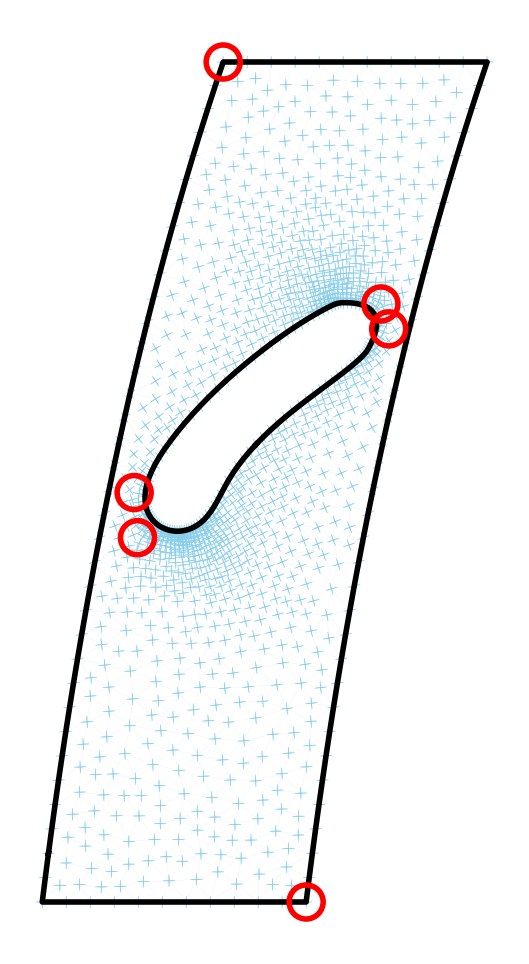
\includegraphics[height=0.74\textheight]{step06_singularities_hub.png}
    \end{column}
  \end{columns}
\end{frame}
\note{Singularities are the unavoidable irregular points where a perfect quad
grid cannot continue: valence not equal to four. On the hub they sit at the
blade tips. The index counts how much the field turns around the point; the
Poincare-Hopf theorem says all indices must sum to the Euler characteristic,
so the topology is constrained, not arbitrary. Red rings mark the final
partition singularities.}

% ---------------------------------------------------------------------------
\begin{frame}{Step 4 --- Streamline Integration}
  \begin{columns}[T]
    \begin{column}{0.58\textwidth}
      \[
        \mathbf{p}_{n+1}=\mathbf{p}_n+\tfrac12(\mathbf{k}_1+\mathbf{k}_2),\quad
        \mathbf{k}_1=h\,\mathbf{v}(\mathbf{p}_n),\ \mathbf{k}_2=h\,\mathbf{v}(\mathbf{p}_n+\mathbf{k}_1)
      \]
      \begin{itemize}
        \item Trace field lines (\emph{separatrices}) out of the singularities
        \item 2nd-order Runge--Kutta--Heun; stable near singular points
        \item Stop on a wall, another singularity, or a corner
      \end{itemize}
      \vspace{0.5em}
      \srcline{\texttt{StreamlineGenerator\_v2}; Kowalski 2015 (Prop.~9:
               index $+1\!\to\!3$ arms, $-1\!\to\!5$ arms)}
    \end{column}
    \begin{column}{0.42\textwidth}
      \centering
      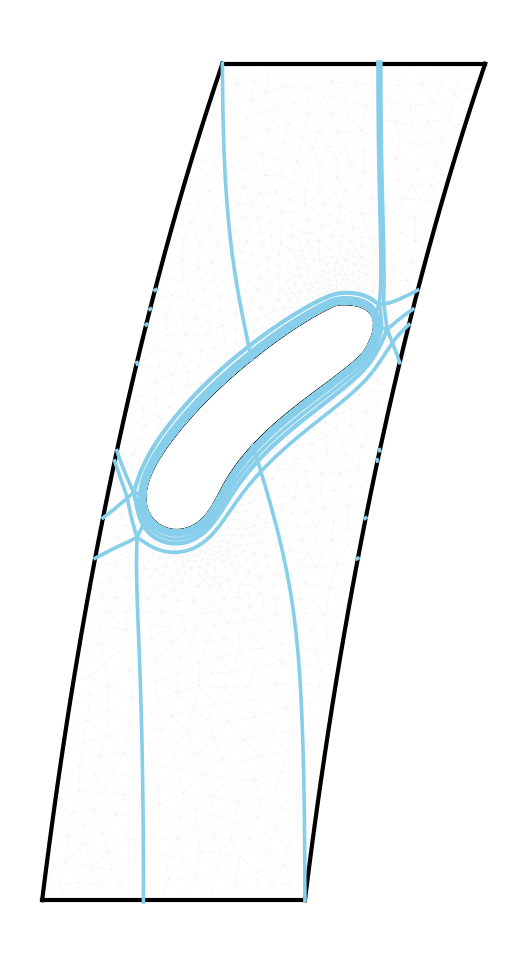
\includegraphics[height=0.74\textheight]{step07_streamline_integration_hub.png}
    \end{column}
  \end{columns}
\end{frame}
\note{From every singularity we shoot curves along the field: the separatrices,
the future block edges. Integration is Runge-Kutta-Heun, a predictor-corrector
that stays stable near the stiff singular points. Curves end on a wall, a
singularity, or a corner. Blue are the separatrices, black the domain walls.}

% ---------------------------------------------------------------------------
\begin{frame}{Step 5 --- Simplify: Merge \& Split}
  \begin{columns}[T]
    \begin{column}{0.58\textwidth}
      \[
        \gamma_{12}(s)=(1-s)\,\gamma_1(s)+s\,\gamma_2(s)
      \]
      \begin{itemize}
        \item \textbf{Merge} near-duplicate arms at a singularity
              (angle criterion), blended by the formula above
        \item \textbf{Split} at transversal crossings $\rightarrow$ T-junctions
        \item Result: clean, quad-only block boundaries
      \end{itemize}
      \vspace{0.5em}
      \srcline{\texttt{StreamlineMerging},
               \texttt{StreamlineIntersectionSplitter};
               Xiao et al.\ 2020 (Alg.~2)}
    \end{column}
    \begin{column}{0.42\textwidth}
      \centering
      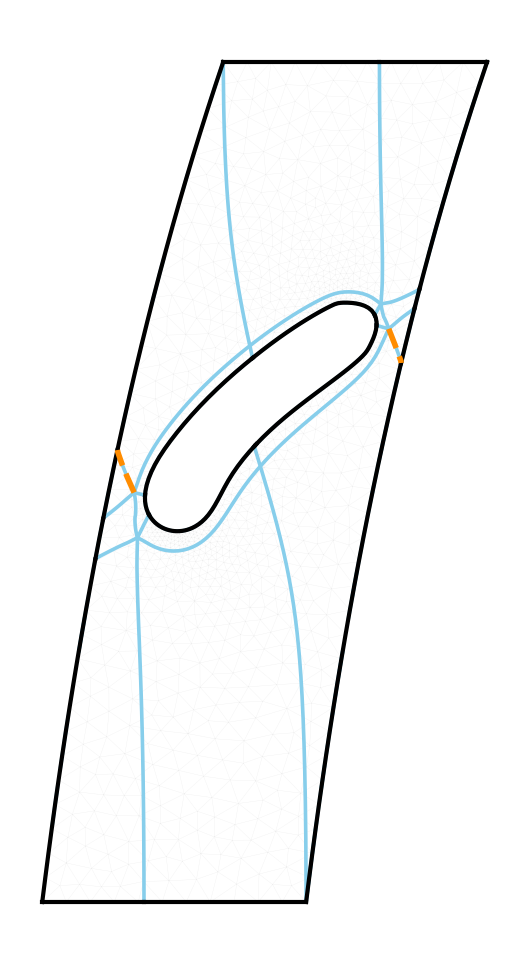
\includegraphics[height=0.74\textheight]{step08_simplification_hub_ta.png}
    \end{column}
  \end{columns}
\end{frame}
\note{Raw streamlines overlap and duplicate. Merging fuses near-duplicate arms
at a singularity when their angle is within the allowed window, blending the
two into one curve. Splitting cuts curves at crossings and inserts T-junctions.
The output is a clean set of block boundaries. Orange dashed: wedge arms the
seam step will delete next.}

% ---------------------------------------------------------------------------
\begin{frame}{Step 6 --- Blocks \& Periodic Seam}
  \begin{columns}[T]
    \begin{column}{0.58\textwidth}
      \begin{itemize}
        \item Extract the quad \textbf{blocks} bounded by the curves
        \item Collapse degenerate 3-sided seam wedges
        \item \textbf{Master--slave} seam: the right wall is the exact
              $+\text{pitch}$ copy of the left --- perfectly periodic
        \item Hanging junctions become T-nodes (variant T-a) or are
              continued into the domain (T-b)
      \end{itemize}
      \vspace{0.5em}
      \srcline{\texttt{collapse\_seam\_wedges},
               \texttt{symmetrize\_seam\_junctions};
               Sauer \& Morsbach (DLR) 2023, sec.~2.7}
    \end{column}
    \begin{column}{0.42\textwidth}
      \centering
      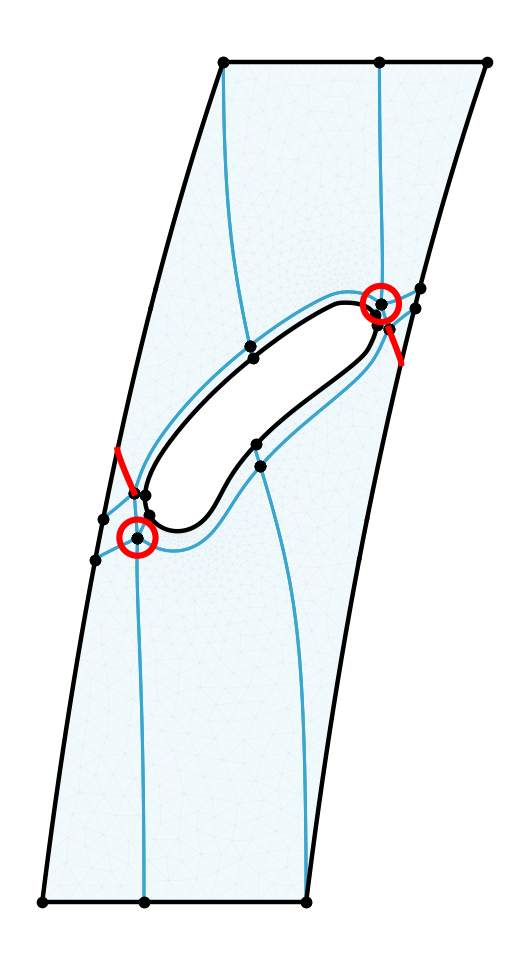
\includegraphics[height=0.74\textheight]{step09_postprocessing_hub_ta.png}
    \end{column}
  \end{columns}
\end{frame}
\note{Now we read off the actual quad blocks enclosed by the curves. Two seam
fixes make it periodic: collapse degenerate three-sided wedges at the wall, and
enforce master-slave conformity so the right theta-wall is literally the left
wall shifted by one pitch. Red marks the wedge streamlines deleted at the seam.
This is the T-a variant with hanging T-nodes.}

% ---------------------------------------------------------------------------
\begin{frame}{Step 7 --- Fill Blocks: Transfinite Interpolation}
  \begin{columns}[T]
    \begin{column}{0.58\textwidth}
      \small
      \[
        \begin{aligned}
          X(u,v)={}&(1-v)S(u)+v\,N(u)+(1-u)W(v)+u\,E(v)\\
          &-\bigl[(1-u)(1-v)c_{00}+u(1-v)c_{10}\\
          &\quad+(1-u)v\,c_{01}+uv\,c_{11}\bigr]
        \end{aligned}
      \]
      \begin{itemize}
        \item \textbf{Coons patch}: a structured grid from 4 block edges
        \item Conforming cell counts $\Rightarrow$ grids match across edges
        \item Wall clustering for the blade boundary layer
      \end{itemize}
      \vspace{0.4em}
      \srcline{\texttt{tfi\_fill}; Coons 1967}
    \end{column}
    \begin{column}{0.42\textwidth}
      \centering
      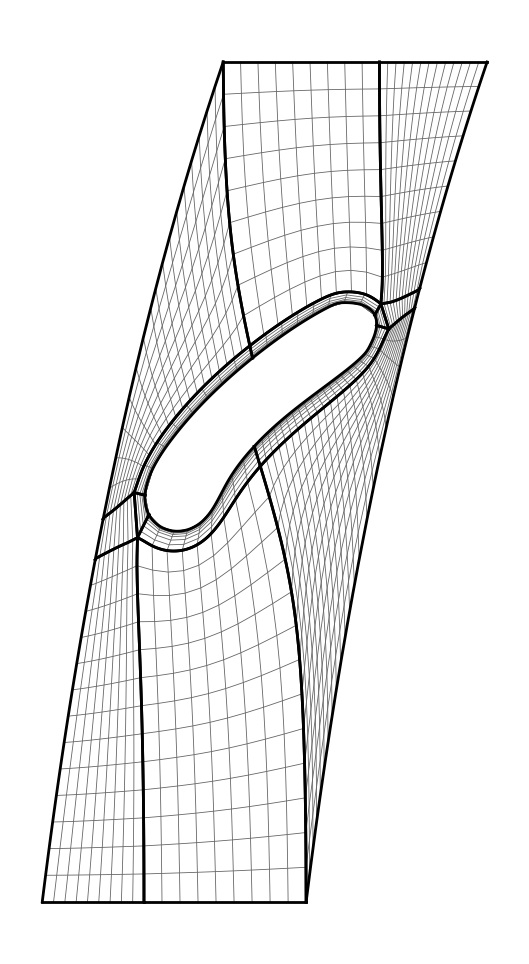
\includegraphics[height=0.74\textheight]{step10_tfi_hub_ta.png}
    \end{column}
  \end{columns}
\end{frame}
\note{Each block is filled with a structured grid via transfinite interpolation,
the Coons patch: blend the four edge curves, subtract the double-counted
corners. Cell counts on opposite sides are solved to match, so neighbouring
grids are conforming. Near the blade we cluster cells for the boundary layer.}

% ---------------------------------------------------------------------------
\begin{frame}{Periodicity Check --- Tiled Passages}
  \centering
  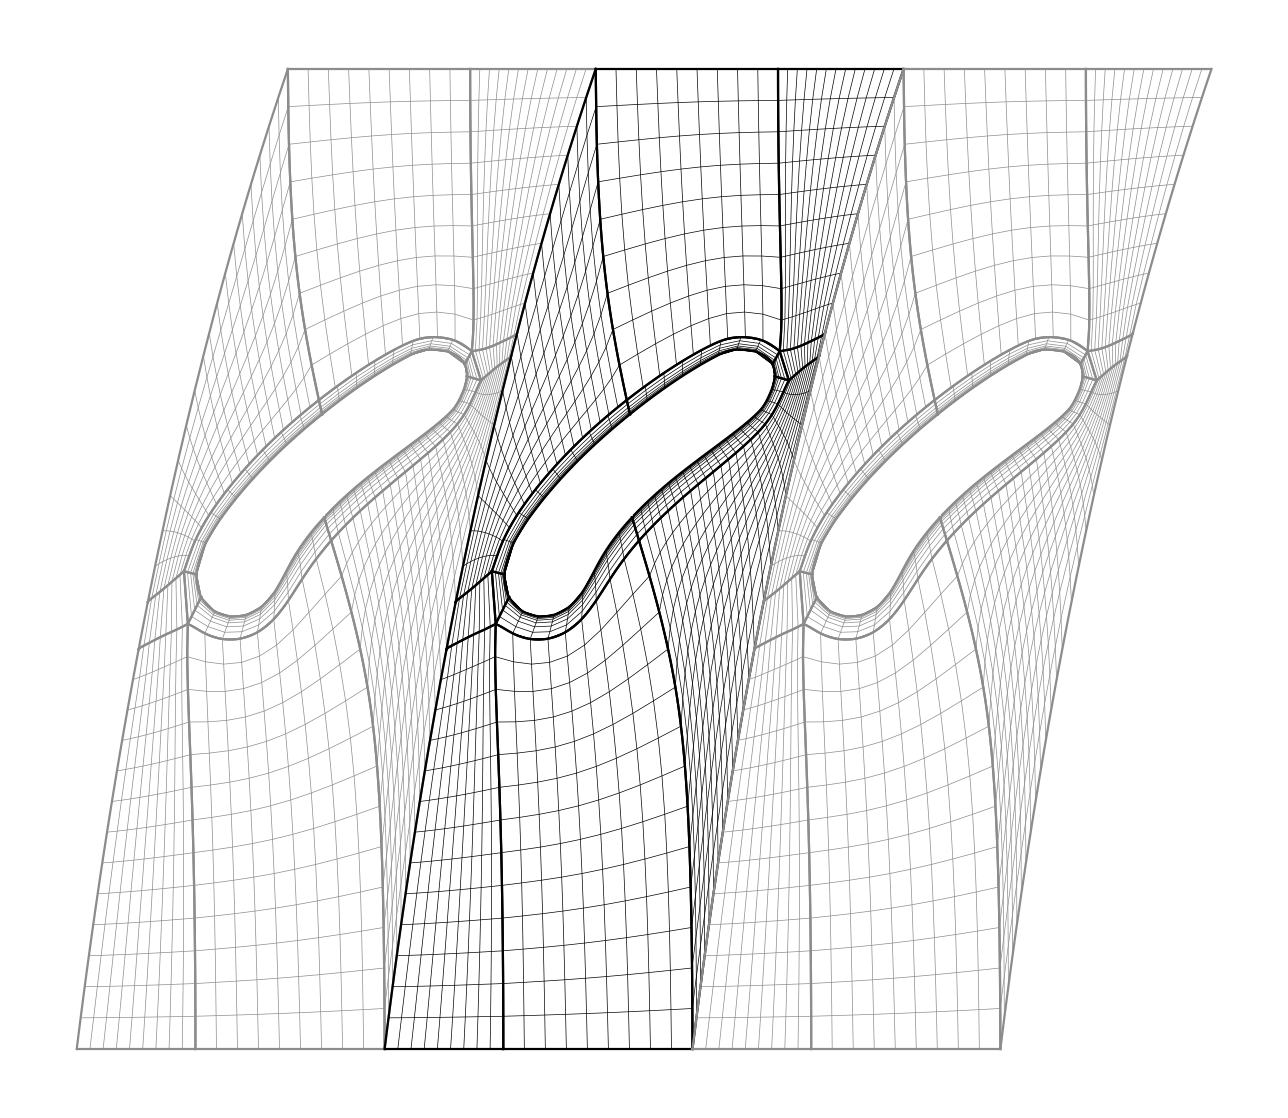
\includegraphics[height=0.72\textheight]{step11_tiled_hub_ta.png}\\
  \srcline{Three passages ($-\text{pitch},\,0,\,+\text{pitch}$): grid points
           coincide across the interior seams --- CFD-conforming periodicity}
\end{frame}
\note{Final sanity check: three passages side by side, shifted by minus pitch,
zero, plus pitch. At the interior seams the grid points of neighbouring copies
land exactly on top of each other -- that is what makes the mesh usable with
periodic CFD boundary conditions.}

% ---------------------------------------------------------------------------
\begin{frame}{Method Comparison}
  \begin{columns}[c]
    \begin{column}{0.33\textwidth}\centering
      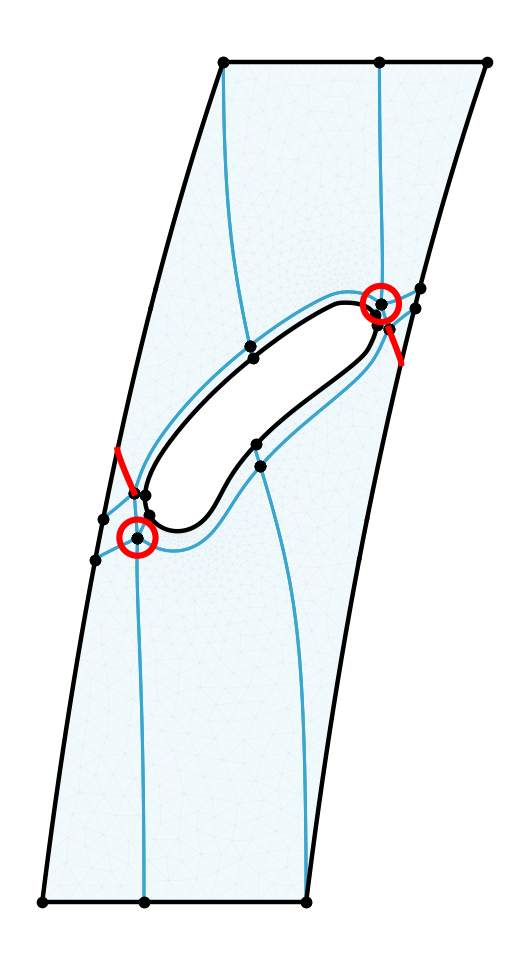
\includegraphics[width=\textwidth]{step09_postprocessing_hub_ta.png}\\
      \textbf{T-a}\\ \srcline{hanging seam T-nodes}
    \end{column}
    \begin{column}{0.33\textwidth}\centering
      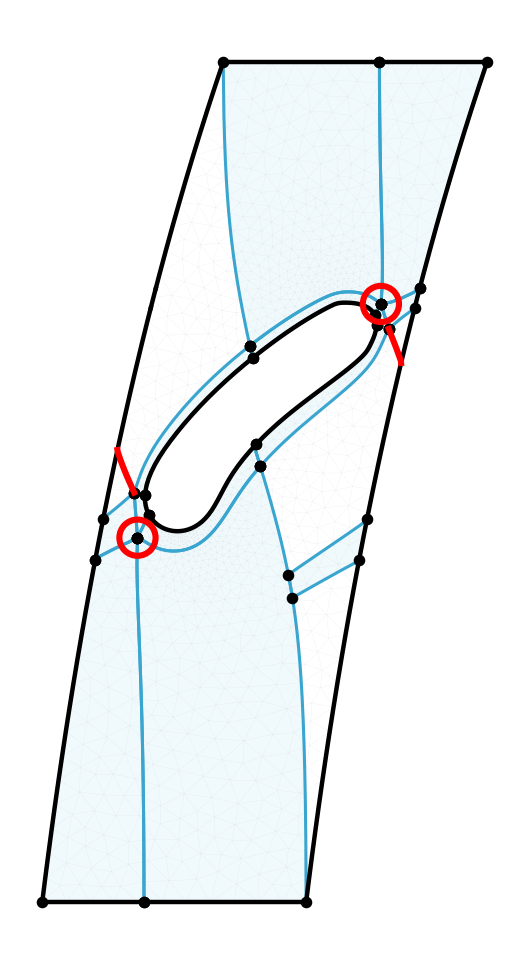
\includegraphics[width=\textwidth]{step09_postprocessing_hub_tb.png}\\
      \textbf{T-b}\\ \srcline{seam edges continued}
    \end{column}
    \begin{column}{0.33\textwidth}\centering
      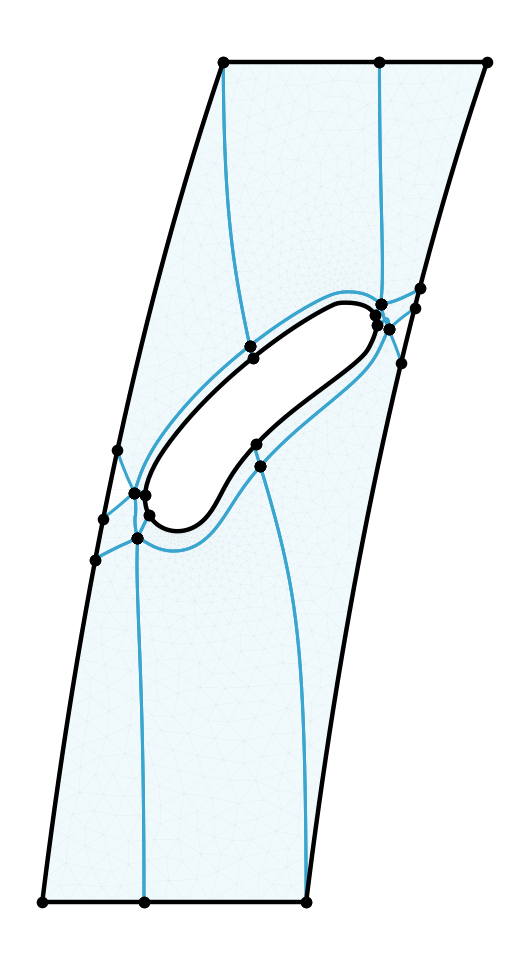
\includegraphics[width=\textwidth]{step09_postprocessing_hub_xiao.png}\\
      \textbf{Xiao}\\ \srcline{baseline, no seam step}
    \end{column}
  \end{columns}
  \vspace{0.4em}
  \centering\footnotesize
  Same field and separatrices --- the variants differ only in the
  block/seam post-processing.
\end{frame}
\note{Three partition variants from the identical field: T-a keeps hanging
T-nodes at the seam; T-b continues those edges into the domain; Xiao is the
plain 2020 baseline with no seam post-processing. Same separatrices, different
block topology near the seam.}

% ---------------------------------------------------------------------------
\begin{frame}{Summary}
  \begin{itemize}
    \item Fully automatic: raw surface $\rightarrow$ block-structured quad mesh
    \item Cross-field $\rightarrow$ singularities $\rightarrow$ separatrices
          $\rightarrow$ blocks $\rightarrow$ TFI grid
    \item Periodic seam handled by master--slave conformity
    \item Hub works end-to-end; shroud + boundary-layer extraction in progress
  \end{itemize}
\end{frame}
\note{Wrap up: the pipeline is automatic end to end for the hub, produces a
periodic block-structured quad mesh, and is built from well-established
building blocks (direction fields, Xiao topology decomposition, Coons patches).
Open work: the shroud case and pulling in the hex-core boundary-layer quads.}

% ---------------------------------------------------------------------------
\begin{frame}{References}
  \footnotesize
  \begin{itemize}
    \item F.~Kn\"oppel, K.~Crane, U.~Pinkall, P.~Schr\"oder.
          \emph{Globally Optimal Direction Fields.} ACM SIGGRAPH 2013.
    \item J.~Xiao et al.
          \emph{Robust topology decomposition of 2D domains.} 2020 (Alg.~2).
    \item N.~Kowalski et al.
          \emph{Block-structured quad meshing / PL-domain blocking.} 2015.
    \item T.~Sauer, C.~Morsbach (DLR).
          \emph{Automated blocking for turbomachinery.} 2023, sec.~2.7.
    \item S.~A.~Coons.
          \emph{Surfaces for Computer-Aided Design of Space Forms.} 1967.
    \item M.~Reberol et al.
          \emph{Quasi-structured quadrilateral meshing in Gmsh.}
    \item J.~F.~Thomas, J.~F.~Middlecoff.
          \emph{Elliptic grid generation with control functions.} 1980.
  \end{itemize}
\end{frame}

% ---------------------------------------------------------------------------
\appendix
\begin{frame}{Appendix --- Labeled Diagnostics}
  \begin{columns}[c]
    \begin{column}{0.33\textwidth}\centering
      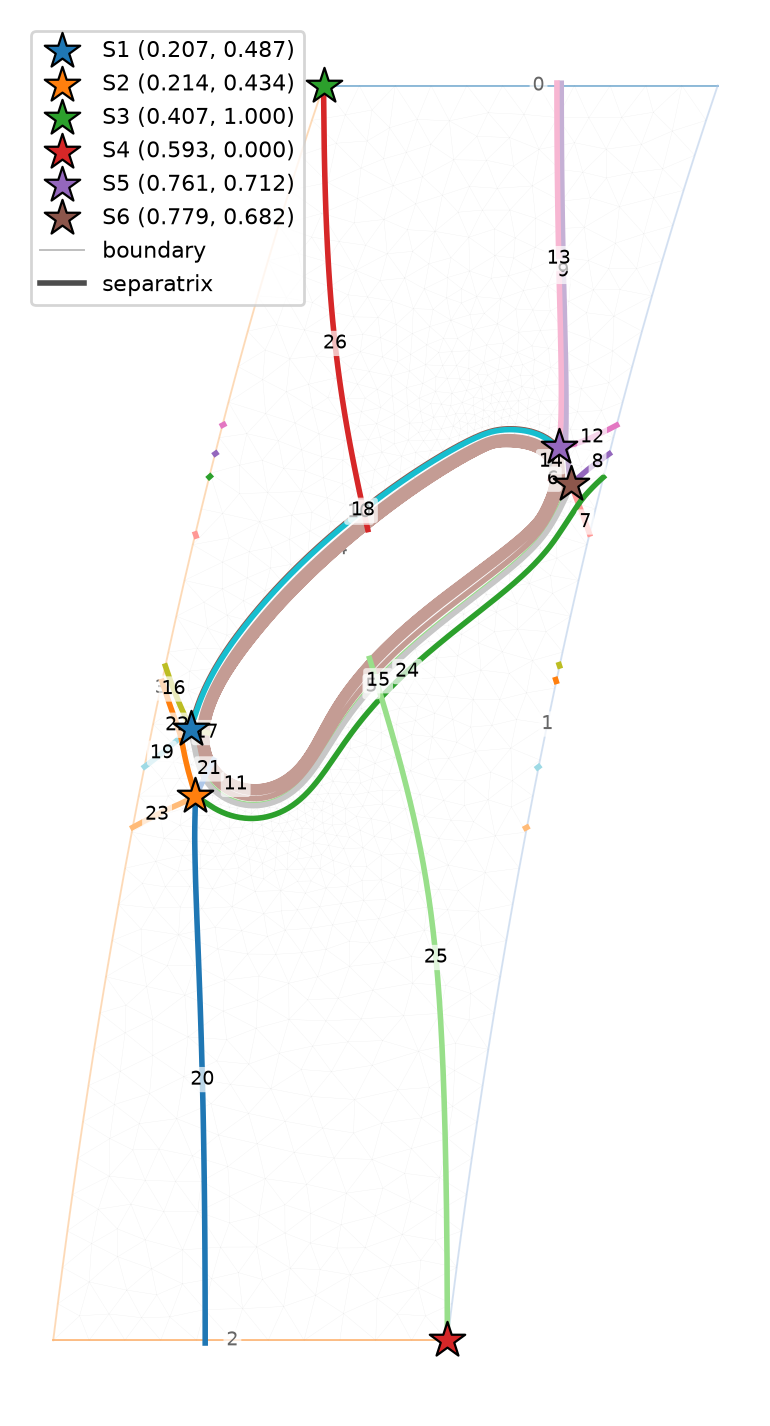
\includegraphics[width=\textwidth]{step07_streamline_integration_hub_labeled.png}\\
      \srcline{separatrices indexed}
    \end{column}
    \begin{column}{0.33\textwidth}\centering
      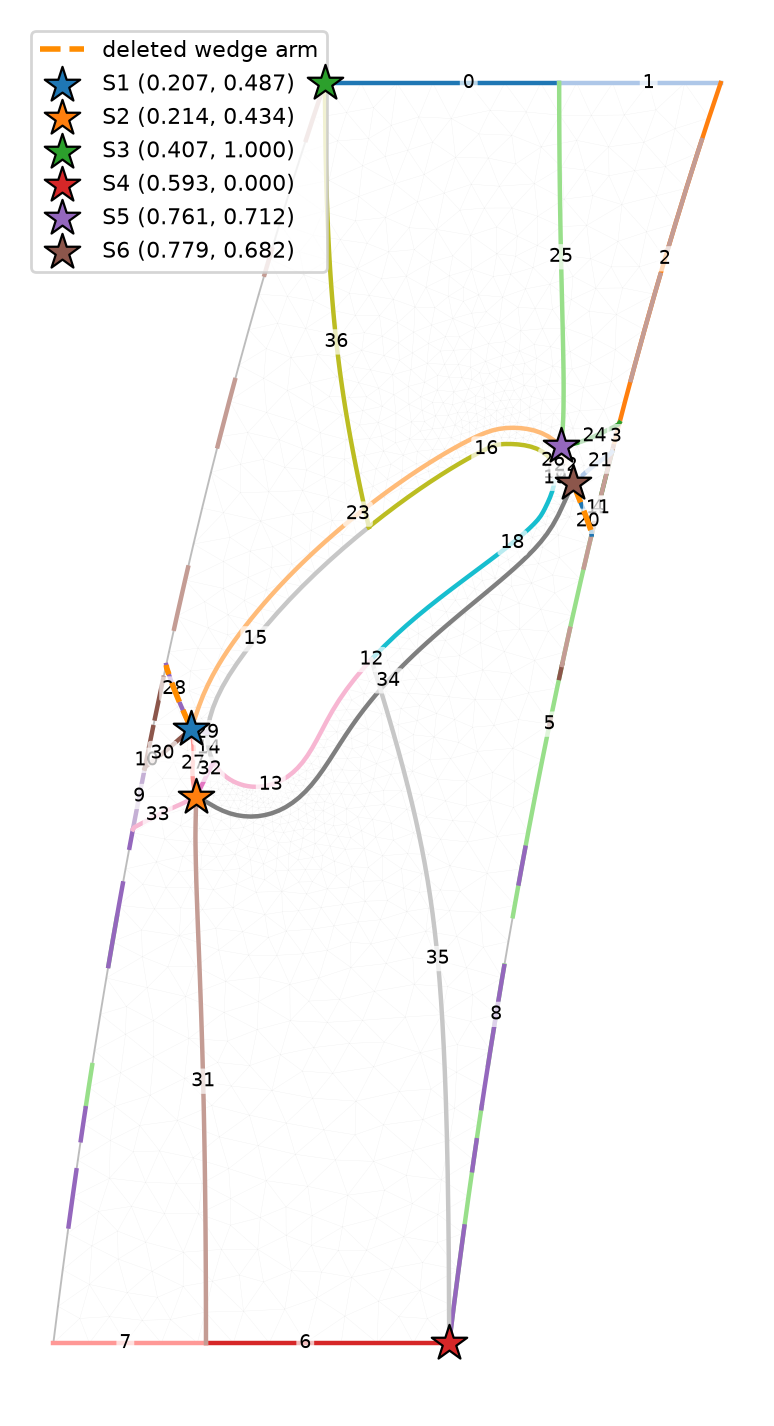
\includegraphics[width=\textwidth]{step08_simplification_hub_ta_labeled.png}\\
      \srcline{merge state indexed}
    \end{column}
    \begin{column}{0.33\textwidth}\centering
      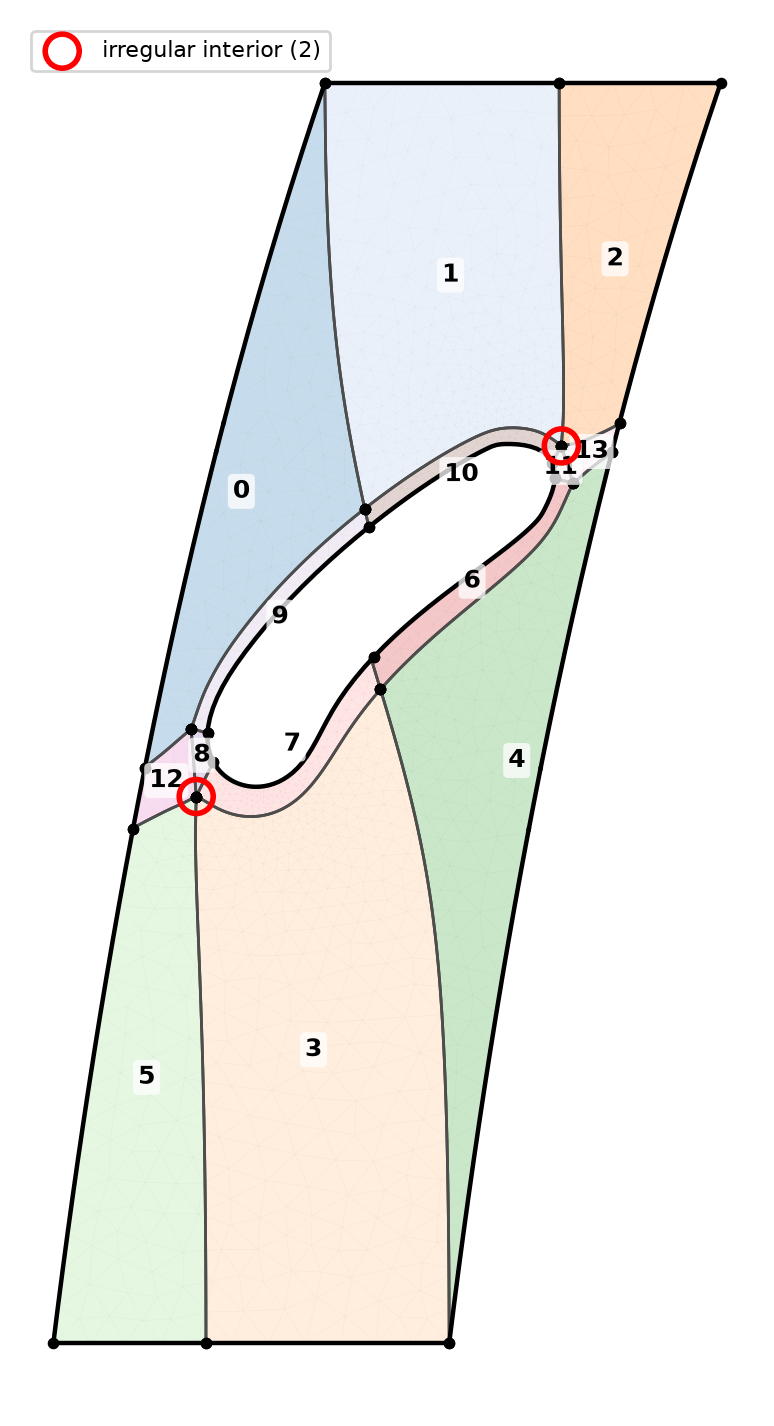
\includegraphics[width=\textwidth]{step09_postprocessing_hub_ta_labeled.png}\\
      \srcline{blocks numbered}
    \end{column}
  \end{columns}
\end{frame}

\end{document}
